\chapter{GSM}

\section{Overview}

GSM (Global System for Mobile Communications, originally Groupe Sp\'ecial 
Mobile), is a very popular standard that describes protocols for second 
generation (2G) digital cellular networks used by mobile phones. GSM networks 
usually operate in the 900 MHz, 1800 MHz or 1900 MHz bands. It supports a full
data rate of 9.6 kbits/sec or 14.4 kbits/sec using better codecs.


\section{System Architecture}

A GSM Public Land Mobile Network (PLMN) consists of at least one Service Area
managed by a Mobile Switching Center (MSC) connected to the Public Switched 
Telephone Network  (PSTN).

\begin{figure}
\centering
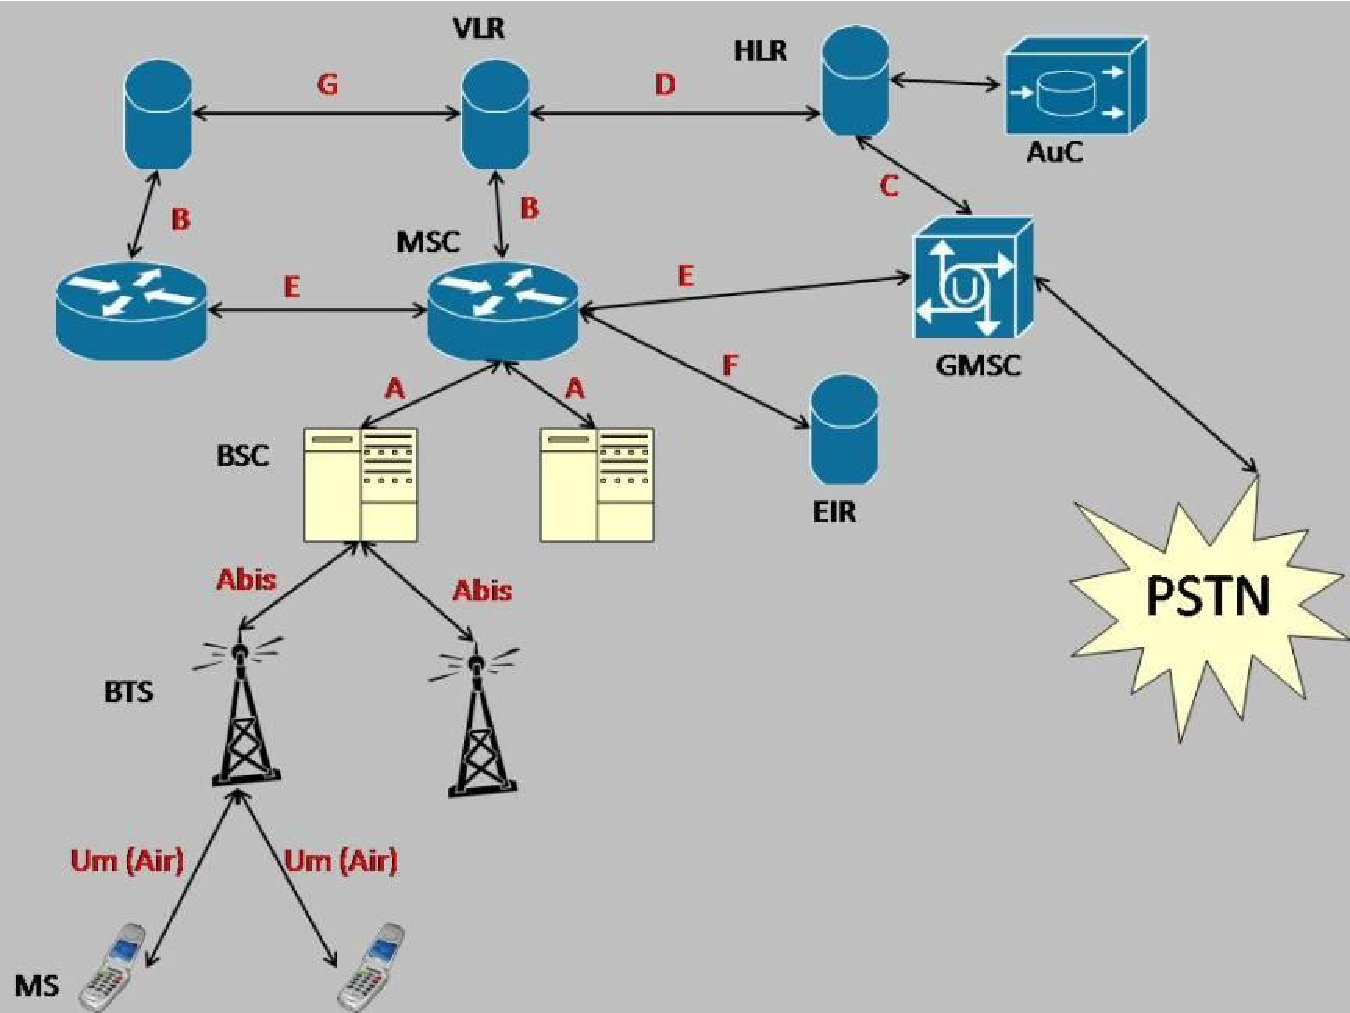
\includegraphics[scale=0.5]{gsmNetwork}
\caption[GSM PLMN architecture]{The architecture of a GSM Public Land Mobile 
Network (PLMN) {\cite{gnuradioFullNet}}}
\end{figure}

The network structure can be divided into the following discrete sections:
\begin{itemize}[noitemsep,topsep=0pt,parsep=0pt,partopsep=0pt]
\item Base Station Subsystem
\item Network and Switching Subsystem
\item Operation Subsystem
\end{itemize}


\subsection{Base Station Subsystem (BSS)}

A base station subsystem consists of
\begin{itemize}[noitemsep,topsep=0pt,parsep=0pt,partopsep=0pt] 
\item a Base Station Controller (BSC) and
\item at least one Base Transceiver Station (BTS) for Mobile Stations (MS).
A mobile station can be a cell phone, or any electronic equipment such as a 
Personal Digital Assistant (PDA) with a phone interface.
\end{itemize}

The area served by a BTS is called a Network Cell. One or more BTSs
are managed by a BSC.  A group of BSSs can be managed as a Location 
Area (Location Area) provided all those BSSs are being managed by the same 
MSC.


\begin{figure}
\centering
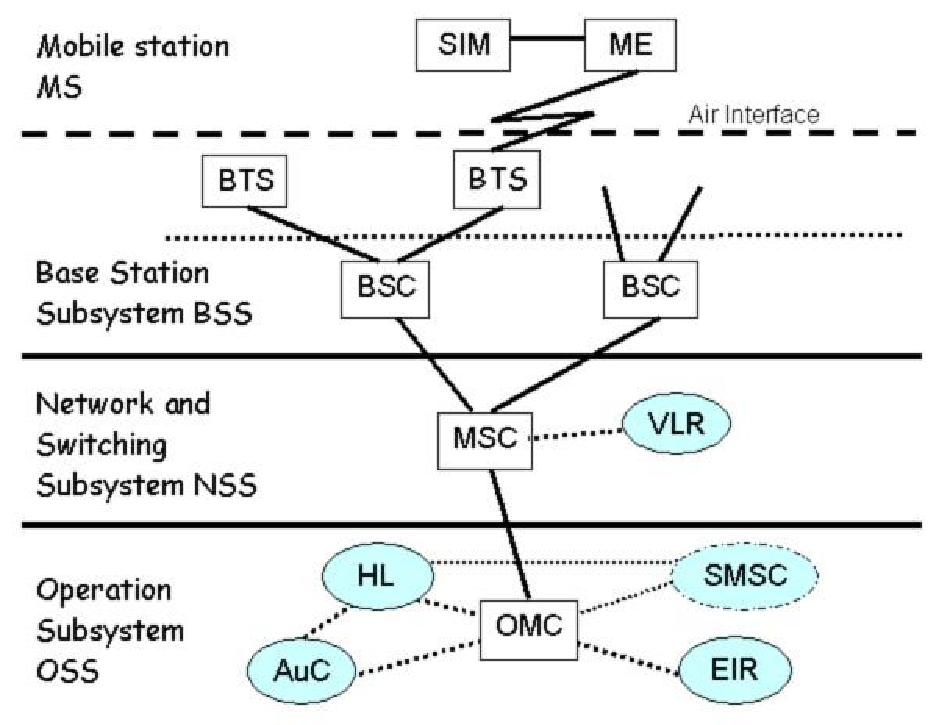
\includegraphics[scale=0.4]{archMSCServiceArea}
\caption[Network architecture for a single MSC Service Area]{The GSM network 
architecture for a single MSC controlled Service Area {\cite{arcadaFi}}.}
\end{figure}


An MSC may also be connected via a Gateway MSC (GMSC) to other MSCs or the
PSTN with the Integrated Services Digital Network (ISDN) option. The 
Inter-Working Function (IWF) of a GMSC makes it possible to connect the 
circuit switched data paths of a GSM network with the PSTN/ISDN.

\subsection{Network and Switching Subsystem (NSS)}

The NSS is made up of an MSC and a Visitor Location Register (VLR). An MSC 
\begin{itemize}[noitemsep,topsep=0pt,parsep=0pt,partopsep=0pt]
\item sets up, controls and shuts down connections
\item handles call charges
\item manages additionals services like call forwarding, call blocking, etc.
\end{itemize}

A VLR contains all the subscriber data and location data of the phones being 
served by the accompanying MSC. The VLR also maintains data about the SIMs 
that do not belong to the network but have roamed into the network. The area 
served by an MSC is called a MSC/VLR service area.

\subsection{The Operation Subsystem (OSS)}

The OSS consists of the Operation and Maintenance Center (OMC), the 
Authentication Center (AuC), the Home Location Register (HLR) and the 
Equipment Identity Register (EIR).

The OSS is responsible for
\begin{itemize}[noitemsep,topsep=0pt,parsep=0pt,partopsep=0pt]
\item network management functions like service provisioning, network 
configuration, fault management, etc.
\item billing calls
\item administering subscribers
\end{itemize}

The AuC controls all the encryption algorithms used for verifying the SIMs. 
The EIR contains the serial numbers of all the MSs (mobile phones) being 
served. The HLR contains the subscriber data and location data of all the 
SIMs in different parts of the network.



\section{Protocol Architecture}
The data communication protocols in a GSM network are implemented to work over
the bearer\footnote{A bearer data channel is a channel that carries call 
content i.e.
one that does not carry signaling.} data channel. 
The GSM protocol architecture is structured into three independent planes:
\begin{itemize}[noitemsep,topsep=0pt,parsep=0pt,partopsep=0pt]
 \item user plane
 \item control plane
 \item management plane
\end{itemize}

The user plane defines protocols for handling the voice and user data. 
At the Um interface, the traffic control channel (TCH) is used to carry the 
user data.

The control plane defines protocols for controlling connections by using 
signalling data.
The signalling data are carried over logical channels called Dm-channels 
(wireless analog of the D-channels for wired interface).
The spare capacities of the Dm-channels are used for carrying user data.
Eventually all logical channels have to multiplexed onto the physical channel.

The management plane takes care of the coordination between different planes.
It also manages functions related to the control and/or user planes.
The management plane handles things like network configuration, network fault,
etc.


\subsection{Signalling Transmission}
In GSM, the network nodes exchange signaling information with each other to
establish, control and terminate connections.
The various interfaces in a GSM network are:
\begin{itemize}[noitemsep,topsep=0pt,parsep=0pt,partopsep=0pt]
 \item MS-BTS: Um
 \item BTS-BSC: Abis
 \item BSC-MSC: A
 \item MSC-VLR: B
 \item MSC-HLR: C
 \item VLR-HLR: D
 \item MSC-MSC: E
 \item MSC-EIR: F
 \item VLR-VLR: G
\end{itemize}

The Um interface is the only interface that uses the wireless physical medium 
for carrying signals. The rest of the interfaces all use wired and digital 
mediums.

\subsubsection{\uppercase{Data Link Layer (Layer 2) protocols}}

\textbf{Link Access Protocol on Dm-channel (LAPDm)} is a layer 2 protocol that
provides safe, reliable connections to layer 3 protocols. It is a 
wireless-adapted version of 
 the standard Link Access Protocol on D-channel (LAPD) of ISDN. It works in 
 two modes: Unacknowledged and Acknowledged. In Unacknowledged mode it 
 operates without acknowledgement,
 without error correction and without flow control. While in acknowledged 
 mode, it asserts acknowledgement, error correction is done by resending and 
 flow is controlled.
 
 
 \textbf{Message Transfer Part (MTP)} is the standard ISDN message transport 
 part of Signaling System 7 (SS7). The networking layers covered by MTP cannot
 be mapped
 one-to-one to the OSI model\footnote{Operation Systems Interconnection 
 model}. But it covers layer 1, layer 2 and parts of layer 3 from the OSI 
 model. The parts of layer 3
 not covered by MTP are covered by Signalling Connection Control Part (SCCP).

\subsubsection{\uppercase{Network Layer (Layer 3) protocols}}

\textbf{Radio Resource Management (RR)} is a protocol that sets up, manages 
and terminates
 radio link channels. It is involved in measuring radio field strength, 
 signal quality etc.
 It manages handover, modulation scheme, co-channel interference, etc. The 
 goal is to 
 utilize the limited spectral resources efficiently.
 

\textbf{Mobility Management (MM)} manages mobility of the mobile stations 
(MS). This protocol is used by the MS to communicate directly with the MSC 
bypassing the BSS. It works over an already established
 RR connection. It handles stuff like TMSI reallocation, authentication, 
 IMSI attach/detach, roaming, location update procedure, etc.
 
 
 \textbf{Call Management (CM)} protocol consists of the following parts:
 \begin{itemize}[noitemsep,topsep=0pt,parsep=0pt,partopsep=0pt]
  \item \textit{Call Control (CC)} sets up, manages and ends calls. For each 
  call a CC instance is created in the MS and another one in the MSC. CC 
  instances 
  communicate over already established MM and RR connections.
  \item \textit{Short Message Service (SMS)} works over already established 
  MM, RR and LAPDm connections.
  \item \textit{Supplementary Services (SS)} provide upper layers the access 
  to GSM supplementary services like call forwarding, call barring, etc. 
 \end{itemize}


\textbf{Signal Connection Control Part (SCCP)} is a SS7 protocol that provides
routing, flow control, connection-orientation, error correction facilities 
etc. It
 works at the A-interface.
 
 
\textbf{Base Station System Application Part (BSSAP)} is a signaling protocol
at the A interface supported by MTP and SCCP.
 \begin{itemize}[noitemsep,topsep=0pt,parsep=0pt,partopsep=0pt]
  \item \textit{Direct Transfer Application Part (DTAP)} handles signaling 
  between the MS and the MSC.
  \item \textit{Base Station System Management Application Part (BSSMAP)} 
  transfers management information from the BSC to the MSC.
  \item \textit{Base Station System Operation and Management Application Part 
  (BSSOMAP)} transports network management information from
  OMC to BSC.
 \end{itemize}


\textbf{Mobile Application Part (MAP)} is an SS7 application-layer protocol 
for the various nodes in a GSM network.
 It provides facilities such as:
  \begin{itemize}[noitemsep,topsep=0pt,parsep=0pt,partopsep=0pt]
   \item roaming support via location update, IMSI attach/detach, 
   authentication
   \item call handling
   \item subscriber tracing
   \item SMS
   \item supplementary services
  \end{itemize}



